\documentclass{article}
\usepackage{graphicx}
\usepackage{float}
\usepackage{hyperref}
\usepackage{listings}
%\usepackage[latin1]{inputenc} 
%\usepackage[T1]{fontenc}
%\usepackage{english}
\title{Batch and Stream Processing: Realtime Analysis of Big Data}
\date{}
\author{Marcel Stolin \\ marcelpascal.stolin@studenti.unitn.it}

\def\Eq#1{\eqref{#1}}
\def\Sec#1{Section~\ref{#1}}
\def\Ex#1{Example~\ref{#1}}
\def\Chap#1{Chapter~\ref{#1}}
\def\Part#1{Part~\ref{#1}}
\def\Fig#1{Figure~\ref{#1}}
\def\Lst#1{Listing~\ref{#1}}
\def\Tab#1{Table~\ref{#1}}
\def\Alg#1{Algorithm~\ref{#1}}
\def\Page#1{Page~\pageref{#1}}

% Listings
%\definecolor{codegreen}{rgb}{0,0.6,0}
%\definecolor{codegray}{rgb}{0.5,0.5,0.5}
%\definecolor{codepurple}{rgb}{0.58,0,0.82}
%\definecolor{backcolour}{rgb}{0.95,0.95,0.92}
%\lstdefinestyle{codestyle}{
%    backgroundcolor=\color{backcolour},   
%    commentstyle=\color{codegreen},
%    keywordstyle=\color{magenta},
%    numberstyle=\tiny\color{codegray},
%    stringstyle=\color{codepurple},
%    basicstyle=\ttfamily\footnotesize,
%    breakatwhitespace=false,         
%    breaklines=true,                 
%    captionpos=b,                    
%    keepspaces=true,                 
%    numbers=left,                    
%    numbersep=5pt,                  
%    showspaces=false,                
%    showstringspaces=false,
%    showtabs=false,                  
%    tabsize=2,
%    frame=lines
%}
%\lstset{style=codestyle}

\begin{document}


\maketitle


\begin{abstract}
Since the beginning of Big Data, batch processing was the most popular choice for processing large amounts of generated data. These existing processing technologies are not suitable to process the large amount of data we face today. Research works developed a variety of technologies that focus on stream processing. Stream processing technologies bring significant performance improvements and new opportunities to handle Big Data. In this paper, we discuss the differences of batch and stream processing and we explore existing batch and stream processing technologies. We also explain the new possibilities that stream processing make possible.
\end{abstract}

% Contents
\section{Part 1}\label{sec:01_part1}

\subsection{Introduction}\label{subsec:01_part1_intro}
% Intro to the HTTP server
In the second lecture of the course, an implementation of a basic HTTP server with the name \textit{TinyHttpd} was introduced.
The functionality of \textit{TinyHttpd} is limited to opening \texttt{.html} files and delivering the content via the HTTP 1.1 protocol to the client.


% Problem statement
The task of part 1 of the first assignment, is to extend the \textit{TinyHttpd} implementation by implementing the functionality to launch an external process. Therefore, the client sends a request via the URL \path{http://localhost:8000/process/reverse?par1=ROMA}. Then, the server executes an external Java process, which reverses the string \texttt{ROMA}, given in the query \texttt{?par1=ROMA}, and responses the result (\texttt{AMOR}) of the external Java process to the client via HTTP 1.1.


% Domain description
Given the above mentioned task description, the following steps have to be implemented:
\begin{enumerate}
\item Create a Java application, called \textit{StringReverser}, which takes a valid String as input and returns the reversed string
\item Extend the \textit{TinyHttpd} implementation to launch external processes when requested by client via the URL \path{http://localhost:8000/process/PROCESS_NAME?PROCESS_PARAMETERS}.
\item Execute the requested process on the server and deliver the process output to the client via the HTTP protocol.
\end{enumerate}


\newpage
\subsection{Conceptual Design}\label{subsec:01_part1_design}
Given the problem statement introduced in \Sec{subsec:01_part1_intro}, a new application called \textit{StringReverser} needs to be implemented, and the \textit{TinyHttpd} server has to be extended in a way to launch an external Java process.

\subsubsection{StringReverser}\label{subsubsec:01_part1_design_stringreverser}
% Design of the StringReverser
The \textit{StringReverser} application is a simple terminal application. It takes any valid String as an input and returns the reversed String as the output. It can be executed via the console. For example, the command \texttt{\$ java -jar StringReverser.jar ROMA} should responses the string \textit{AMOR}.

\subsubsection{TinyHttpd}\label{subsubsec:01_part1_design_tinyhttpd}
% Extension of TinyHttpd
Whenever the client makes a request via the URL \path{http://localhost:8000/process/PROCESS_NAME?PROCESS_PARAMETERS}, the server is supposed to start an external Java process, waits for the output of the process, and responses the process output to the user.
% URL
The client has the possibilities to specify which process has to be executed. Given the URL \path{http://localhost:8000/process/reverse?par1=ROMA}, the user explicitly requests to launch the \textit{reverse} process with the given query \texttt{par1=ROMA} as the process input.
% Input
It is important to mention, that each process takes individual parameters as input. For the above mentioned \texttt{StringReverser}, only the value of the first parameter in the given query is important. All other parameters, and the parameter key, are therefore ignored.


\newpage
\subsection{Implementation}\label{subsec:01_part1_impl}
To implement the given conceptual design mentioned in \Sec{subsec:01_part1_design}, OpenJDK 17\footnote{JDK 17 - \url{https://openjdk.java.net/projects/jdk/17/} (Accessed: 02/10/2021)} is used.

\subsubsection{StringReverser}\label{subsubsec:01_part1_impl_stringreverser}
% Implementation of StringReverser
The application \textit{StringReverser} is a simple Java project. It is composed of a single Java class called \texttt{StringReverser} as shown in \Fig{fig:01_part1_impl_stringreverser_structure}.
% Implementation of StringReverser
The source code is shown in \Lst{lst:01_part1_impl_stringreverser_code}, and it consists of a \texttt{main} method and a method called \texttt{reverseString}.
% The main method
The main method will be executed, when the application is launched via the terminal. Additionally, it checks if the given input string is valid. Otherwise, it will return an error message and exits with system code 0. If the input is a valid string, it will call the \texttt{reverseString} method, and returns the result as the output.
% The reverse method
The \texttt{reverseMethod} is responsible to reverse the given input. To achieve this, it uses the \texttt{StringBuilder}\footnote{StringBuilder - \url{https://docs.oracle.com/javase/7/docs/api/java/lang/StringBuilder.html} (Accessed: 02/10/2021)} class to reverse the String.

% StringReverser project structure
\begin{figure}[h]
\centering
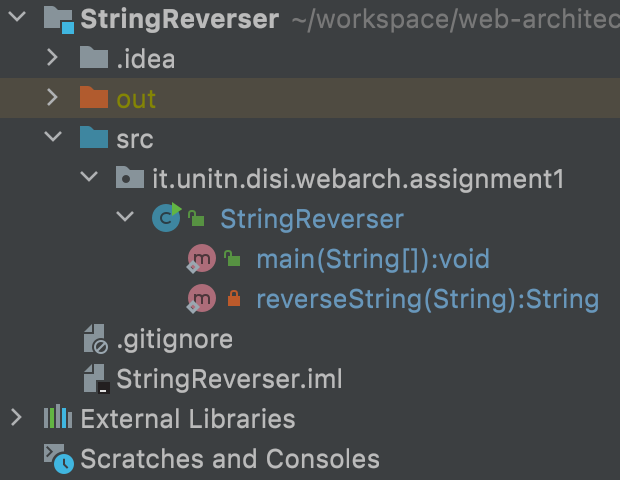
\includegraphics[scale=0.4]{images/StringReverserStrct}
\caption{Project structure of the \texttt{StringReverser} application}
\label{fig:01_part1_impl_stringreverser_structure}
\end{figure}

% Execution
\Fig{fig:01_part1_impl_stringreverser_execution} shows the execution of the \textit{StringReverser} application. The \texttt{.jar} artifact was created using the IntelliJ IDEA\footnote{Create your first Java application - \url{https://www.jetbrains.com/help/idea/creating-and-running-your-first-java-application.html} (Accessed: 02/10/2021)}.
% Failure execution
If the input is invalid, the \texttt{StringReverser} will print an error message to the terminal and exits with system code 0, as shown in \Fig{fig:01_part1_impl_stringreverser_execution_fail}.

% StringReverser execution
\begin{figure}[h]
\centering
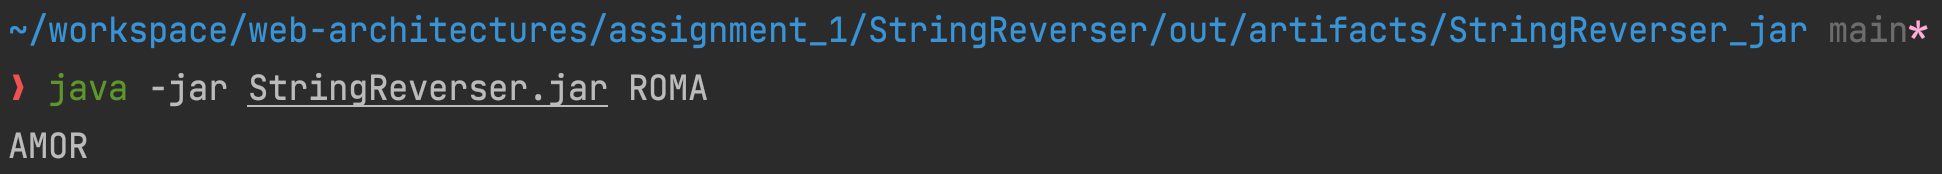
\includegraphics[scale=0.4]{images/StringReverserExec}
\caption{Successful execution of the \textit{StringReverser} application}
\label{fig:01_part1_impl_stringreverser_execution}
\end{figure}

% StringReverser execution fail
\begin{figure}[h]
\centering
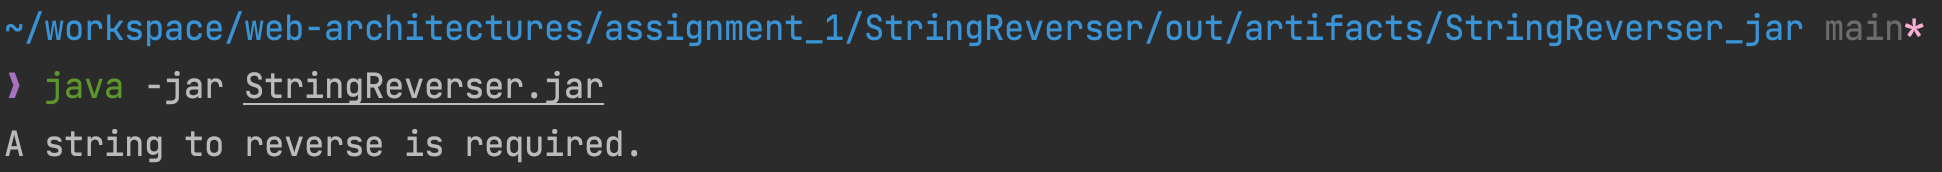
\includegraphics[scale=0.4]{images/StringReverserExecFail}
\caption{Execution of the \textit{StringReverser} application without an input}
\label{fig:01_part1_impl_stringreverser_execution_fail}
\end{figure}

\subsubsection{TinyHttpd}
% Extension of TinyHttpd
The foundation of the \textit{TinyHttpd} project is provided by the Professor. It has to be extended to launch an external Java process, and deliver the process output to the client as a HTTP response.
% The steps
To implement the conceptual design mentioned in \Sec{subsubsec:01_part1_design_tinyhttpd}, the \textit{TinyHttpd} project has to be extended in the following way:
% impl details
\begin{enumerate}
\item Parse the HTTP request to check if a process has been requested
\item Generate the command to execute the requested process
\item Launch an external process, using the generated command
\item Response the process output to the client via HTTP
\end{enumerate}
In the following, the single steps are described in detail.


% Parse request
\paragraph{Step 1:}
The first step of the implementation, is to check if the client requested the execution of a process. Therefore, the HTTP request has to be parsed accordingly. For this task, a new Java class called \texttt{RequestParser} is introduced to the \textit{TinyHttpd} project. The \texttt{RequestParser} class is able to parse a HTTP request into its parts. For example, the request \texttt{GET /process/reverse?param=roma HTTP/1.1} is composed of the HTTP method (\texttt{GET}), the path (\path{/process/reverse?param=roma}), and the HTTP protocol version (\texttt{HTTP/1.1}). Furthermore, the path has an additional query attached (\texttt{?param=roma}). The implementation of the \texttt{RequestParser} class is attached at \Lst{lst:01_part1_impl_tinyhttpd_requestparser}.


% Then start process
After the \texttt{RequestParser} has successfully parsed the clients request, it is possible to check, by using an \texttt{if} statement, if the user requested the path \path{/request/PROCESS_NAME}. If yes, the server executes the requested process, and sends a response accordingly. Otherwise, an error message is sent to the user as shown in \Fig{fig:01_part1_impl_tinyhttpd_invalidprocess}. If no process has been requested, the server tries to open the HTML file according to the given path and responses the HTML content to the client.

% Invalid process
\begin{figure}[h]
\centering
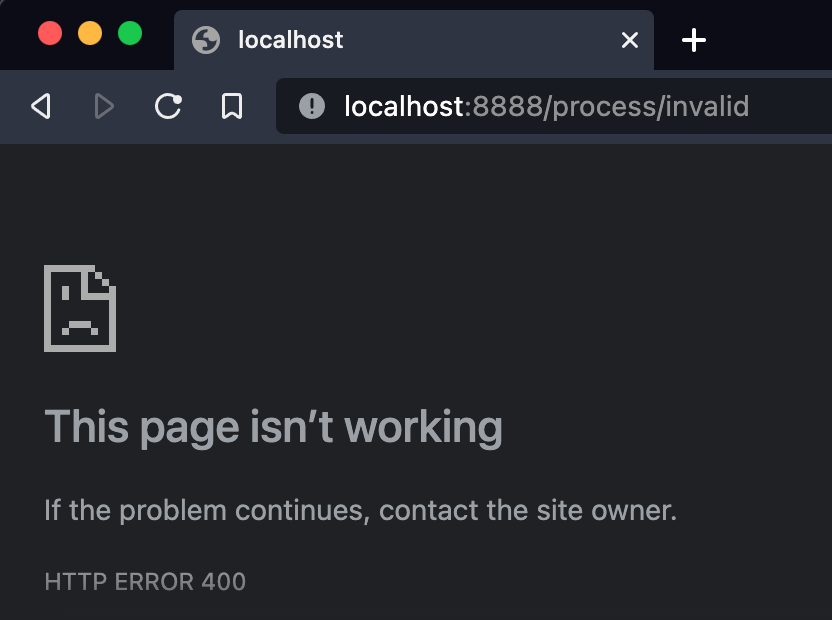
\includegraphics[scale=0.4]{images/invalidProcess}
\caption{Response for an invalid process name}
\label{fig:01_part1_impl_tinyhttpd_invalidprocess}
\end{figure}


% Start the requestes process
\paragraph{Step 2:}
If the client has send a valid request for a process, the next step is to generate the command to launch the requested process. To keep the \textit{TinyHttpd} implementation extensible, a new class called \texttt{CommandFactory} is added to the project, which is implemented using the Factory pattern. The implementation of this class is attached at \Lst{lst:01_part1_impl_tinyhttpd_commandfactory}.
% CommandFactory
The \texttt{CommandFactory} class is responsible to generate the command for the given request. It has a public static method called \texttt{generateCommand}, which takes the requested process name and the query of the request path as arguments. If the given query is invalid, the method will throw an exception and an error message is sent to user as seen in \Fig{fig:01_part1_impl_tinyhttpd_invalidquery}.
% Explain the method
According to the given process name, it generates the command to execute the \texttt{.jar} artifact with the given query as input parameter.
% Example
As example, for the given path \texttt{/process/reverse?param=roma}, the generated command is \texttt{java -jar} \path{/Users/marcel/workspace/web-architectures/assignment_1/MiniHTTPD/jars/StringReverser.jar} \texttt{"roma"}. In addition, the \texttt{CommandFactory} is also responsible for checking, if the requested process is available and if the given query is a valid parameter for the process. If not, it will throw an exception.

% Invalid process
\begin{figure}[h]
\centering
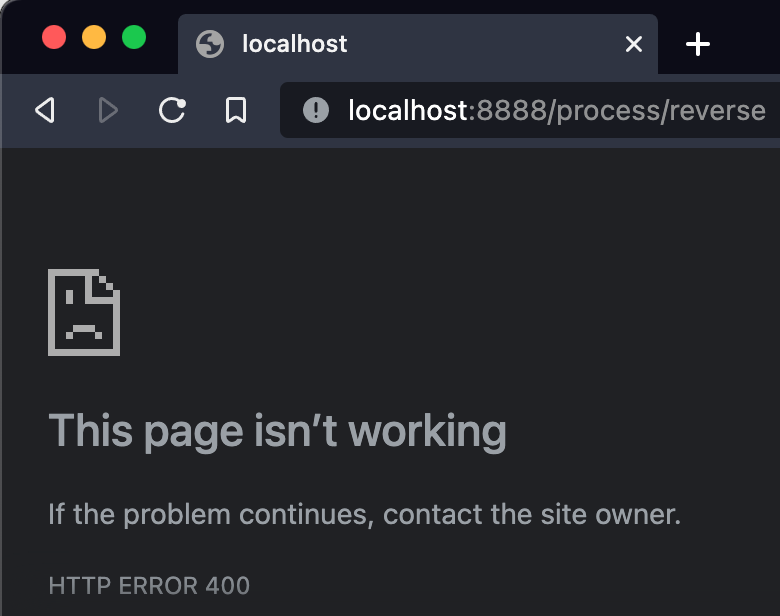
\includegraphics[scale=0.4]{images/invalidQuery}
\caption{Response for an invalid query}
\label{fig:01_part1_impl_tinyhttpd_invalidquery}
\end{figure}


% Launch process
\paragraph{Step 3:}
After the command has been generated, it needs to be executed in a shell. To achieve this, the \texttt{TinyHttpd} class is extended with a new new method called \texttt{launchProcess}. The implementation of this method is available at \Lst{lst:01_part1_impl_tinyhttpd_launchprocess}. This method takes the generated command as an argument and executes it using the \texttt{ProcessBuilder}\footnote{ProcessBuilder - \url{https://docs.oracle.com/javase/7/docs/api/java/lang/ProcessBuilder.html} (Accessed: 02/10/2021)} class.
% How it is executed
The method executes the given command in the bash shell using \texttt{bash -c COMMAND} and returns the process output as a string. It is important, that the process output is returned as a string, instead of printing it directly to the HTTP output stream. The reason is, that the HTTP header of the server response needs the length of the process output.
% Show the execution
\Lst{lst:01_part1_impl_tinyhttpd_implsteps} shows the execution of the \texttt{launchProcess} method and \Fig{fig:01_part1_impl_output} shows the output to the console, after the process has been executed successfully.

% steps implementation
\begin{figure}[h]
\centering
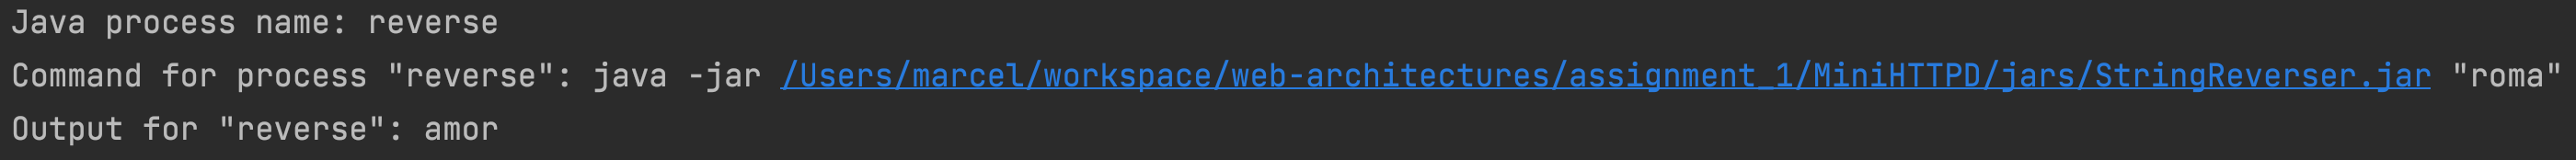
\includegraphics[scale=0.3]{images/implementationOutput}
\caption{Console output after the generated command has been launched successfully}
\label{fig:01_part1_impl_output}
\end{figure}


% Response to the client
\paragraph{Step 4:}
The last step, is to send the process output as a HTTP response to the client.
% How its send
A method called \texttt{sendSuccessResponseHeader} is added to the \textit{TinyHttpd} class, which is responsible to send a \texttt{200 OK} HTTP response. Additionally, the method takes the length of the output as an argument, which was mentioned before, as well as the MIME type of the response content. The implementation of the \texttt{sendSuccessResponseHeader} is attached at \Lst{lst:01_part1_impl_tinyhttpd_sendSuccessResponseHeader}.
% Send
\Lst{lst:01_part1_impl_tinyhttpd_implsteps} shows the whole process of generating the process command, launching the command, and sending the reponse to the client. First a header with the process output length and the MIME type \texttt{text/plain} is written to the output stream, then the process output. \Fig{fig:01_part1_impl_success} shows the response in the browser for a successful process request.

% successful response
\begin{figure}[h]
\centering

\includegraphics[scale=0.6]{images/part1Success}
\caption{A successful process request}
\label{fig:01_part1_impl_success}
\end{figure}

\section{Part 2}\label{sec:02_part2}

\subsection{Introduction}\label{subsec:02_part2_intro}
% Short intro
In addition to the \textit{TinyHttpd}, dynamic pages have been introduced in the lecture. In detail, the Common Gateway Interface (CGI) has been introduced, which is able to spawn processes on the server, and send the result as a HTTP response.
% Problem statement
The task of this part of the assignment, is to create a script, that performs the \textit{StringReverser} application, as introduced in \Sec{subsubsec:01_part1_design_stringreverser}, and responses the result via HTTP. This task is almost equally to the first task (introduced in \Sec{subsec:01_part1_intro}), but rather than extending an existing Java project, a script has to be created which will be launched within the \texttt{cgi-bin} folder of the Apache Web Server.
% Apache
For this task, the Apache Web Server is an requirement and the version XAMPP 7.4.23 for Mac is being used. 

\subsection{Conceptual Design}\label{subsec:02_part2_design}
% What does the script
Given the previously introduced problem statement in \Sec{subsec:02_part2_intro}, a script will be implemented using bash. Therefore, the environment variables can be used, to read details about the HTTP request.
% Procedure
Overall, the script has the same requirements, as the modification of the first task. However, the client can send a request via the url \texttt{http://localhost:80/cgi-bin/run\_reverse\_process.sh?param=ROMA}. Therefore, the use case is limited to the reverse process.

\subsection{Implementation}\label{subsec:02_part2_impl}
% Explain implementation
The implementation of the script is available at \Lst{lst:02_part2_impl_script}.
% Steps
The script is implemented in accordance to the following steps:
\begin{enumerate}
\item Check if the request was send via GET
\item Verify if a query is given
\item Validate the given query
\item If the given query is valid, perform the \textit{StringReverser} Java process and send the process output to the client via HTTP
\end{enumerate}

% First
A simple if statement is used to check if the request was send via the GET method, otherwise an error message is sent. The request method is available via the environment variable \texttt{\$REQUEST\_METHOD}.


% Query
In the next step, the query has to be validated, which is saved in the environment variable \texttt{\$QUERY\_STRING}. If \texttt{\$QUERY\_STRING} is either not set or empty, an error message is sent by the script, which is illustrated in \Fig{fig:01_part2_impl_failure1}.

% failure 1 response
\begin{figure}[h]
\centering
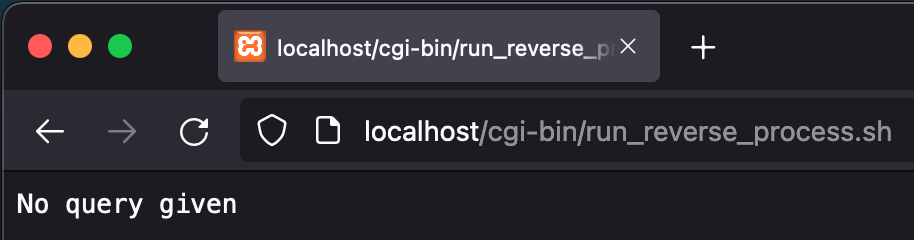
\includegraphics[scale=0.6]{images/part2Failure1}
\caption{The error message if no query is provided}
\label{fig:01_part2_impl_failure1}
\end{figure}

% Get the string
After the query string has been validated accordingly, the value of the first parameter has to be extracted. This is done by splitting the query string into its single parts. Next, the script checks if the value of the first parameter is valid. If not, an error message is sent to client, as illustrated in \Fig{fig:01_part2_impl_failure2}.

% failure 2 response
\begin{figure}[h]
\centering
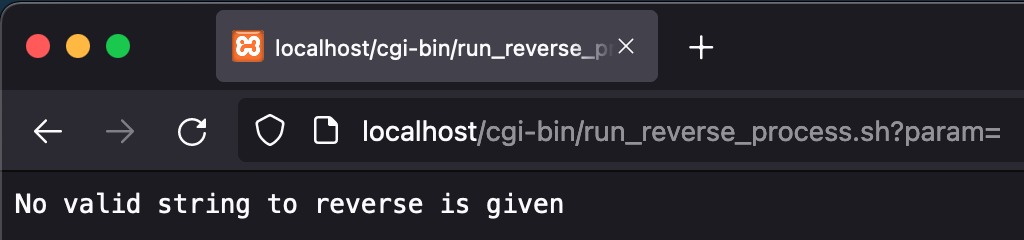
\includegraphics[scale=0.6]{images/part2Failure2}
\caption{The error message if the query is invalid}
\label{fig:01_part2_impl_failure2}
\end{figure}

% Now execute
The last step, is to execute the \textit{StringReverser} application by executing it via the command \texttt{java -jar ARTIFACT STRING\_TO\_REVERSE}. Therefore, the generated \texttt{.jar} artifact is placed in the \texttt{cgi-bin/} directory of the Apache installation. After the process has been executed successfully, the output is send to the client as a HTTP response with the MIME type \texttt{text/plain}. This is shown in \Fig{fig:01_part2_impl_success}.

% successful response
\begin{figure}[h]
\centering

\includegraphics[scale=0.6]{images/part2Success}
\caption{A successful process request using the cgi-bin script}
\label{fig:01_part2_impl_success}
\end{figure}

\subsection{Conclusion}\label{subsec:02_part2_concl}
Was war einfacher? PArt1 oder Part 2

% References
\bibliographystyle{plain}
\bibliography{mybib}

% Appendix
\pagebreak
\appendix
\phantomsection
\section{Part 1}

\subsection{Implementation}

\subsubsection{StringReverser}

\begin{lstlisting}[label=lst:01_part1_impl_stringreverser_code, caption=CLI command to start a GitLab runner in a Docker container, language=java, numbers=none]
package it.unitn.disi.webarch.assignment1;

public class StringReverser {

    public static void main(String[] args) {
        if (args.length >= 1) {
            String text = args[0];

            if (text != null) {
                String reversedString = reverseString(text);
                System.out.println(reversedString);
            }
        } else {
            System.out.println("A string to reverse is required.");
            System.exit(0);
        }
    }

    /**
     * This method reverses the given string.
     *
     * @param text
     * @return Reversed text
     */
    private static String reverseString(String text) {
        StringBuilder stringBuilder = new StringBuilder(text);
        stringBuilder.reverse();
        return stringBuilder.toString();
    }

}
\end{lstlisting}

\subsubsection{TinyHttpd}

\begin{lstlisting}[label=lst:01_part1_impl_tinyhttpd_requestparser, caption=CLI command to start a GitLab runner in a Docker container, language=java, numbers=none]
package it.unitn.disi.webarch.tinyhttpd.utils;

import java.util.StringTokenizer;

public class RequestParser {

    private String request;
    private String method;
    private String protocol;
    private String fullPath;
    private String path;
    private String queryString;

    /**
     * The RequestParser is able to parse an HTTP request
     * into its single parts.
     *
     * @param request
     */
    public RequestParser(String request) throws Exception {
        this.request = request;
        this.parseRequest();
        this.parsePath();
    }

    private void parseRequest() throws Exception {
        StringTokenizer tokenizer = new StringTokenizer(this.request);
        if (tokenizer.countTokens() < 3) {
            throw new Exception("The request \"" + this.request + "\" is invalid");
        }

        this.method = tokenizer.nextToken();
        this.fullPath = tokenizer.nextToken();
        this.protocol = tokenizer.nextToken();
    }

    private void parsePath() {
        StringTokenizer tokenizer = new StringTokenizer(this.fullPath, "?");

        this.path = tokenizer.nextToken();
        if (tokenizer.hasMoreTokens()) {
            this.queryString = tokenizer.nextToken();
        }
    }

    public String getMethod() {
        return this.method;
    }

    public String getProtocol() {
        return this.protocol;
    }

    public String getPath() {
        return this.path;
    }

    public String getQueryString() {
        return this.queryString;
    }
}
\end{lstlisting}

\begin{lstlisting}[label=lst:01_part1_impl_tinyhttpd_commandfactory, caption=CLI command to start a GitLab runner in a Docker container, language=java, numbers=none]
package it.unitn.disi.webarch.tinyhttpd.utils;

import java.util.StringTokenizer;

public class CommandFactory {

    /**
     * Generates the command for the given process name.
     *
     * @param process Name of the requested process
     * @param parameters Probably the query string
     * @return Command as string
     * @throws Exception If the process name is unknown
     */
    public static String generateCommand(String process, String parameters) throws Exception {
        if (process.equals("reverse")) {
            return generateReverseProcessCommand(parameters);
        } else {
            throw new Exception("No process called \"" + process + "\" available");
        }
    }

    private static String generateReverseProcessCommand(String parameters) throws Exception {
        StringTokenizer paramTokenizer = new StringTokenizer(parameters, "&");
        // first check if there are any parameters
        if (!paramTokenizer.hasMoreTokens()) {
            throw new Exception("No parameters given. The reverse process needs at least one parameter");
        }
        String firstParam = paramTokenizer.nextToken();
        String[] paramKeyValue = firstParam.split("=");
        if (paramKeyValue.length >= 2) {
            // We need at least 2 elements
            String textToReverse = paramKeyValue[1];
            String artifactPath = System.getProperty("user.dir") + "/jars/StringReverser.jar";
            String command = "java" + " -jar " + artifactPath + " \"" + textToReverse + "\"";

            return command;
        } else {
            throw new Exception("No valid parameter input given for parameters \"" + parameters + "\"");
        }
    }

}
\end{lstlisting}

\begin{lstlisting}[label=lst:01_part1_impl_tinyhttpd_launchprocess, caption=CLI command to start a GitLab runner in a Docker container, language=java, numbers=none]
private String launchProcess(String command) throws Exception {
    ProcessBuilder processBuilder = new ProcessBuilder();
    processBuilder.command("bash", "-c", command);
    Process process = processBuilder.start();

    StringBuilder output = new StringBuilder();
    BufferedReader reader = new BufferedReader(
            new InputStreamReader(process.getInputStream()));

    String line;
    while ((line = reader.readLine()) != null) {
        output.append(line + "\n");
    }

    return output.toString();
}
\end{lstlisting}

\begin{lstlisting}[label=lst:01_part1_impl_tinyhttpd_sendSuccessResponseHeader, caption=CLI command to start a GitLab runner in a Docker container, language=java, numbers=none]
private void sendSuccessResponseHeader(int responseLength, String mimeType) {
    ps.print("HTTP/1.1 200 OK\r\n");
    ps.print("Content-Length: " + responseLength + "\r\n");
    ps.print("Content-Type: " + mimeType + "\r\n");
    ps.print("\r\n");
}
\end{lstlisting}

\section{Part 2}

\subsection{Implementation}

\begin{lstlisting}[label=lst:02_part2_impl_script, caption=CLI command to start a GitLab runner in a Docker container, language=bash, numbers=none]
#!/bin/sh

send_response () {
  echo "Content-type: text/plain; charset=iso-8859-1"
  echo "Content-Length: ${#1}"
  echo
  echo $1
}


# Check if the request method is GET
if [ $REQUEST_METHOD == "GET" ]; then
  # Check if query is given
  if [ ! $QUERY_STRING ]; then
    send_response "No query given"
  else
    # Parse query
    saveIFS=$IFS
    IFS='=&'
    params=($QUERY_STRING)
    IFS=$saveIFS
    STRING_TO_REVERSE=${params[1]}

    # Check if the given parameter is valid
    if [ ! $STRING_TO_REVERSE ]; then
      send_response "No valid string to reverse is given"
    else
      REVERSE_JAVA_ARTIFACT="$(pwd)/StringReverser.jar"
      REVERSED_STRING=$(java -jar $REVERSE_JAVA_ARTIFACT $STRING_TO_REVERSE)

      send_response $REVERSED_STRING
    fi
  fi
else
  send_response "Only GET requests are allowed"
fi
\end{lstlisting}


\end{document}